\documentclass{standalone}

\usepackage[latin1]{inputenc}
\usepackage{amsmath}
\usepackage{amssymb}
\usepackage{amsthm}

\usepackage{tikz}
\usetikzlibrary{shapes,arrows,shapes.geometric,calc,patterns}

%% generates a tightly fitting border around the work
%\usepackage[active,tightpage]{preview}
%\PreviewEnvironment{tikzpicture}
%\setlength\PreviewBorder{0.5mm}
%%\renewcommand\PreviewBbAdjust{-\PreviewBorder 1mm -1.15mm -0.85mm}

\usepackage{color}

%\pagestyle{empty}

\begin{document}

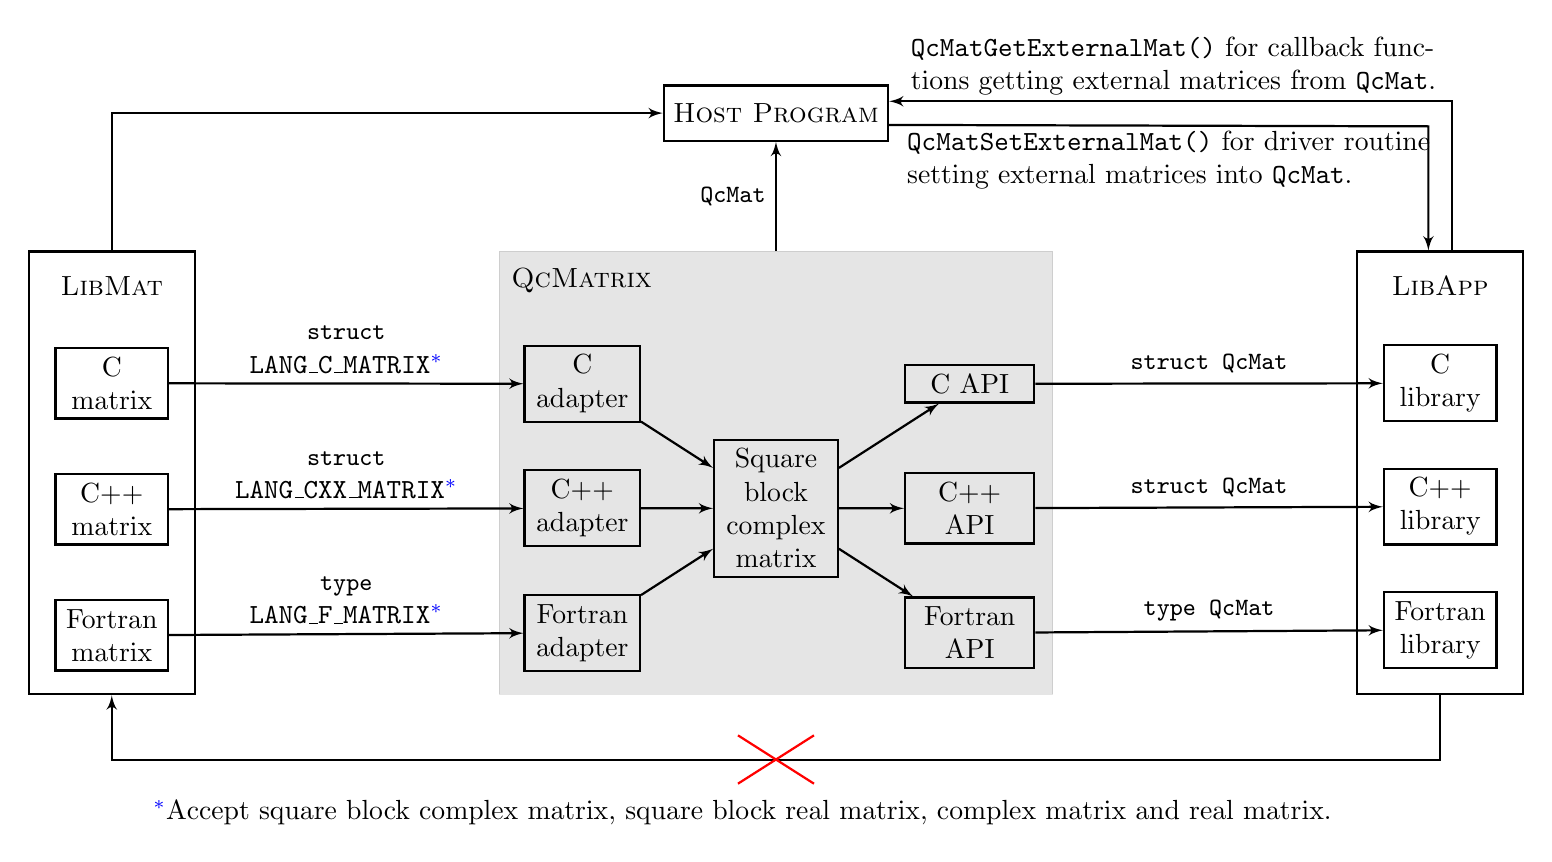
\begin{tikzpicture}[scale=0.75, auto, thick, node distance=40]
  % host programs
  \node [color=black, rectangle, draw, text badly centered, sharp corners, %
    minimum height=20, minimum width=55] (HostProg) {\textsc{Host Program}};
  % QcMatrix
  \node [below of=HostProg, fill=black, opacity=0.1, color=black, rectangle, %
    very thin, draw, text badly centered, sharp corners, minimum height=16em, %
    minimum width=20em, node distance=130] (QcMatrix) {~};
  \node at ($(QcMatrix.north west)-(-1.4,0.5)$) {\textsc{QcMatrix}};
  \node at ($(QcMatrix.base)-(0,0.6)$) [color=black, rectangle, draw, text badly centered, %
    sharp corners, minimum height=2, text width=3.8em, node distance=0] (BlockCmplx) %
    {Square block complex matrix};
  % QcMatrix adapters
  \node [left of=BlockCmplx, color=black, rectangle, draw, text badly centered, %
    sharp corners, minimum height=2, text width=3.5em, node distance=70] %
    (CxxAdapter) {C++ adapter};
  \draw [color=black, -latex'] (CxxAdapter)--(BlockCmplx);
  \node [above of=CxxAdapter, color=black, rectangle, draw, text badly centered, %
    sharp corners, minimum height=2, text width=3.5em, node distance=45] %
    (CAdapter) {C adapter};
  \draw [color=black, -latex'] (CAdapter)--(BlockCmplx);
  \node [below of=CxxAdapter, color=black, rectangle, draw, text badly centered, %
    sharp corners, minimum height=2, text width=3.5em, node distance=45] (FAdapter) %
    {Fortran adapter};
  \draw [color=black, -latex'] (FAdapter)--(BlockCmplx);
  % QcMatrix APIs
  \node [right of=BlockCmplx, color=black, rectangle, draw, text badly centered, %
    sharp corners, minimum height=2, text width=4em, node distance=70] %
    (CxxAPI) {C++ API};
  \draw [color=black, -latex'] (BlockCmplx)--(CxxAPI);
  \node [above of=CxxAPI, color=black, rectangle, draw, text badly centered, %
    sharp corners, minimum height=2, text width=4em, node distance=45] %
    (CAPI) {C API};
  \draw [color=black, -latex'] (BlockCmplx)--(CAPI);
  \node [below of=CxxAPI, color=black, rectangle, draw, text badly centered, %
    sharp corners, minimum height=2, text width=4em, node distance=45] (FAPI) %
    {Fortran API};
  \draw [color=black, -latex'] (BlockCmplx)--(FAPI);
  % external matrix libraries
  \node [left of=QcMatrix, rectangle, draw, text badly centered, sharp corners, %
    minimum height=16em, minimum width=6em, node distance=240] (LibMat) {~};
  \node at ($(LibMat.north)-(0,0.6)$) {\textsc{LibMat}};
  % C matrix
  \node at ($(LibMat.north)-(0,2.25)$) [color=black, rectangle, draw, text badly centered, %
    sharp corners, minimum height=2, text width=3.4em, node distance=0] (CLibMat) %
    {C matrix};
  \draw [color=black, -latex'] (CLibMat) %
    edge node[align=center, midway] %
    {\small\texttt{struct}\\\texttt{LANG\_C\_MATRIX}\color{blue}$^{*}$}(CAdapter);
  % C++ matrix
  \node at ($(CLibMat.north)-(0,2.75)$) [color=black, rectangle, draw, text badly centered, %
    sharp corners, minimum height=2, text width=3.4em, node distance=0] (CxxLibMat) %
    {C++ matrix};
  \draw [color=black, -latex'] (CxxLibMat) %
    edge node[align=center, midway] %
    {\small\texttt{struct}\\\texttt{LANG\_CXX\_MATRIX}\color{blue}$^{*}$}(CxxAdapter);
  % Fortran matrix
  \node at ($(CxxLibMat.north)-(0,2.75)$) [color=black, rectangle, draw, text badly centered, %
    sharp corners, minimum height=2, text width=3.4em, node distance=0] (FLibMat) %
    {Fortran matrix};
  \draw [color=black, -latex'] (FLibMat) %
    edge node[align=center, midway] %
    {\small\texttt{type}\\\texttt{LANG\_F\_MATRIX}\color{blue}$^{*}$}(FAdapter);
  % application libraries
  \node [right of=QcMatrix, rectangle, draw, text badly centered, sharp corners, %
    minimum height=16em, minimum width=6em, node distance=240] (LibApp) {~};
  \node at ($(LibApp.north)-(0,0.6)$) {\textsc{LibApp}};
  % C library
  \node at ($(LibApp.north)-(0,2.25)$) [color=black, rectangle, draw, text badly centered, %
    sharp corners, minimum height=2, text width=3.4em, node distance=0] (CLibApp) %
    {C library};
  \draw [color=black, -latex'] (CAPI) %
    edge node[midway]{\small\texttt{struct QcMat}}(CLibApp);
  % C++ library
  \node at ($(CLibApp.north)-(0,2.75)$) [color=black, rectangle, draw, text badly centered, %
    sharp corners, minimum height=2, text width=3.4em, node distance=0] (CxxLibApp) %
    {C++ library};
  \draw [color=black, -latex'] (CxxAPI) %
    edge node[midway]{\small\texttt{struct QcMat}}(CxxLibApp);
  % Fortran library
  \node at ($(CxxLibApp.north)-(0,2.75)$) [color=black, rectangle, draw, text badly centered, %
    sharp corners, minimum height=2, text width=3.4em, node distance=0] (FLibApp) %
    {Fortran library};
  \draw [color=black, -latex'] (FAPI) %
    edge node[midway]{\small\texttt{type QcMat}}(FLibApp);
  % connections
  \draw [-latex'] (LibMat.north) |- ($(HostProg.west)-(1,0)$) -- (HostProg.west);
  \draw [color=black, -latex'] (QcMatrix) %
    edge node[midway]{\small\texttt{QcMat}}(HostProg);
  \draw [color=black, -latex'] ($(LibApp.north)+(0.2,0)$) |- %
    node[at end, align=left, xshift=86.5, yshift=27, text width=20em] %
    {\texttt{QcMatGetExternalMat()} for callback functions getting external matrices from \texttt{QcMat}.} %
    ($(HostProg.east)+(1,0.2)$) -- ($(HostProg.east)+(0,0.2)$);
  \draw [color=black, -latex'] ($(HostProg.east)-(0,0.2)$) -- %
    node[at start, align=left, xshift=106.5, yshift=-27, text width=20em] %
    {\texttt{QcMatSetExternalMat()} for driver routine setting external matrices into \texttt{QcMat}.} %
    ($(LibApp.north)-(0.2,-2.1)$) -| ($(LibApp.north)-(0.2,0)$);
  % reduces coupling
  \draw [color=black, -latex'] (LibApp.south) |- node[near end]{~}($(LibApp.south)-(1,1.1)$)-- %
    ($(LibMat.south)-(0,1.1)$) -- (LibMat.south);
  \node [cross out, draw=red, text width=2em, text height=1em] at ($(QcMatrix.south)-(0,1.1)$) {~};
  % notes
  \node [text width=45em, text ragged] at ($(QcMatrix.south)-(0,2)$) {\color{blue}$^{*}$%
    \color{black}Accept square block complex matrix, square block real matrix, complex %
    matrix and real matrix.};
\end{tikzpicture}

\end{document}
